\documentclass[11pt, ngerman, fleqn, DIV=15, headinclude, BCOR=2cm]{scrreprt}

\usepackage{../../header}

\usepackage{placeins}
\usepackage[maxfloats=50]{morefloats}

\usepackage{csquotes}

\usepackage{tikz}
\usetikzlibrary{chains}
\usetikzlibrary{shapes.geometric}

\tikzset{device/.style={
                rectangle,
                minimum size=6mm,
                draw=black
            },
            monitor/.style={
                rectangle,
                rounded corners=2mm,
                minimum size=6mm,
                draw=black
            },
        }

\usepackage{pgfplots}
\pgfplotsset{
    compat=1.9,
    width=0.8\linewidth,
    xticklabel style={/pgf/number format/use comma},
    yticklabel style={/pgf/number format/use comma},
}
\usepgfplotslibrary{polar}

\usepgfplotslibrary{external}
\tikzexternalize[mode=list and make]
\tikzsetexternalprefix{Abbildung-}

\DeclareSIUnit{\skt}{SKT}

\usepackage{booktabs}

\hypersetup{
    pdftitle=
}

\subject{Praktikumsprotokoll}
\title{Höhenstrahlung}
\subtitle{Versuch P518 -- Universität Bonn}
\author{
    Martin Ueding \\ \small{\href{mailto:mu@martin-ueding.de}{mu@martin-ueding.de}}
    \and
    Lino Lemmer \\
    \small{\href{mailto:l2@uni-bonn.de}{l2@uni-bonn.de}}
}

\date{\daterange{2014-07-02}{2014-07-03}}

\publishers{Tutor: Michael Lupberger}

\begin{document}

\maketitle

\begin{abstract}
    Wir vermessen die Energie- und Winkelabhängigkeit der Höhenstrahlung.
    Außerdem bestimmen wir die Lebensdauer der Myonen.
\end{abstract}

\tableofcontents

\chapter{Theorie}

\section{Höhenstrahlung}

\begin{figure}[htbp]
    \centering
    \tikzsetnextfilename{cos2}
    \begin{tikzpicture}
        \begin{polaraxis}
            \addplot[black] table {cos2.csv};
        \end{polaraxis}
    \end{tikzpicture}
    \caption{%
        Erwartete Intensitätsverteilung der Höhenstrahlung $\cos(\theta)^2$.
        Dabei ist $\theta$ hier so gewählt, dass $\theta = \SI{0}{\degree}$
        einer Einstrahlung senkrecht zum Erdboden entspricht.
    }
    \label{fig:cos2}
\end{figure}

\section{Standardmodell}

\section{Interaktion von Teilchen mit Materie}

\section{Zerfallsgesetz und Lebensdauer}

\section{Detektoren}

\section{Logische Schaltungen}

\subsection{Constant Fraction Diskriminator (CFD)}

Ein Diskriminator ist ein Gerät, welches nur anspricht, wenn ein eintreffendes
Signal stärker ist, als ein bestimmter Grenzwert (engl. \emph{threshold}).
Trifft ein solches Signal ein, gibt der Diskriminator ein Standardsignal, zum
Beispiel ein Rechtecksignal aus.

Eine Anwendung des Diskriminators ist das Triggern: Trifft ein Signal ein, wird
ein neues, standardisiertes abgegeben. So ist zum Beispiel der zeitliche
Abstand zwischen zwei eintreffenden Signalen zu messen. Wann genau der
Diskriminator triggert, kommt auf die Art an.

Ein CFD triggert, wenn ein bestimmter Anteil der Maximalamplitude erreicht
wird. Dazu wird das einkommende Signal gesplittet, ein Teil wird zeitlich
verzögert, der andere invertiert und um einen Faktor $k$ gedämpft. Anschließend
werden beide Signale wieder addiert. Ein vorher rein positives Signal erhält so
eine Nullstelle, welche durch $k$ bestimmt wird und den Triggerpunkt definiert.

\parencite{Ueding/525}

\section{Vorbereitungsfragen zur Winkelverteilung}

Dies sind die Vorbereitungsfragen aus \parencite[11]{physik512-Anleitung}.

\begin{quote}
    Wie funktionieren Szintillatoren und Photomultiplier? Welche physikalischen
    Prozesse und apparativen Einflüsse bestimmen den zeitlichen Verlauf des
    Photomultiplier-Ausgangssignals? Wie hängt die Pulshöhe von der gewählten
    Hochspannung am Photomultiplier ab?
\end{quote}

% TODO Antwort einfügen.

\begin{quote}
    Wie funktionieren Diskriminator- und Koinzidenz-Schaltungen? Wie sehen die
    jeweiligen Ausgangssignale aus? Wie beeinflusst die Schwellenhöhe eines
    Diskriminators die zeitliche Lage des Ausgangssignals gegenüber dem
    Eingangssignal?
\end{quote}

% TODO Antwort einfügen.

\begin{quote}
    Die Zählrate für jeden einzelnen Zähler betrage etwa 1 Hz am
    Diskriminatorausgang. Wie groß ist die theoretisch zu erwartende Rate der
    Zufallskoinzidenzen für eine der Dreifach- Koinzidenz-Schaltungen zur
    Messung der Winkelverteilung der Höhenstrahlung? Und für die
    Koinzidenz-Schaltung, die zur Messung des Pulshöhenspektrums verwendet
    wird? Wie groß sind jeweils die Totzeiten? Machen Sie einen Vorschlag, wie
    die Rate der Zufallskoinzidenzen für eine der
    Dreifach-Koinzidenz-Schaltungen gemessen werden kann.
\end{quote}

% TODO Antwort einfügen.

\begin{quote}
    Welchen inhaltlichen Zusammenhang haben Bethe-Bloch-Gleichung und
    Landau-Verteilung?
\end{quote}

% TODO Antwort einfügen.

\begin{quote}
    Welche Beiträge hat das Pulshöhenspektrum? Welche physikalischen und
    apparativen Einflüsse bestimmen die Form des Pulshöhenspektrums? Wie
    unterscheiden sich zwei Pulshöhenspektren, wenn diese mit und ohne aktiven
    Gate-Eingang aufgenommen werden?
\end{quote}

% TODO Antwort einfügen.

\begin{quote}
    Wie hängen Pulshöhenspektrum und Schwellenkurve zusammen? Wie ändert sich
    die Form der Schwellenkurve, wenn man die Anzahl der Koinzidenzsignale
    anstelle der Diskriminatorsignale betrachtet?
\end{quote}

% TODO Antwort einfügen.

\begin{quote}
    Welche Funktion erfüllt das in Abbildung 5 gezeigte LabVIEW-Programm?
\end{quote}

% TODO Antwort einfügen.

\section{Vorbereitungsfragen zur Myonenlebensdauer}

Dies sind die Vorbereitungsfragen aus \parencite[14]{physik512-Anleitung}.

\begin{quote}
    Es kommen sowohl Myonen als auch Antimyonen auf der Erdoberfläche an.
    Welcher atom- physikalische Prozeß ist für Myonen möglich, aber nicht für
    Antimyonen? Wie beeinflußt das qualitativ die in diesem Versuch gemessene
    Lebensdauer?
\end{quote}

% TODO Antwort einfügen.

\begin{quote}
    Machen Sie einen Vorschlag, wie man unter Verwendung von Diskriminatoren,
    Verzögerungs- kabeln und Koinzidenz-Schaltungen die START-und STOP-Impulse
    erzeugen kann.
\end{quote}

% TODO Antwort einfügen.

\begin{quote}
    Entwerfen Sie das Blockschaltbild für Messkreis und Monitorkreis.
\end{quote}

% TODO Antwort einfügen.

\begin{quote}
    Können Sie eine andere Gestaltung der Zeitintervalle vorschlagen, die die
    Genauigkeit der Myonlebensdauerbestimmung optimieren würde?
\end{quote}

Die Intervalleinteilung in der Anleitung ist linear. Da ein exponentieller
Abfall in der Kurve zu erwarten ist, werden in den ersten Intervallen mehr
Ereignisse gemessen als in den letzten. Dadurch ist der relative Fehler in den
ersten Intervallen kleiner. Verkleinert man die ersten und streckt dafür die
letzten Intervalle exponentiell, kann man dadurch den relativen Fehler in allen
Intervallen gleich bekommen.

\begin{quote}
    Das aus der Apparatur kommende Start-Signal wird gegenüber dem Stop-Signal
    um ca. 100 ns verzögert. Warum ist das notwendig? Wie wirkt es sich auf das
    Messergebnis aus?
\end{quote}

Diese Verzögerung wurde auch schon in Versuch 525 benutzt, um sicherzustellen,
dass das Start-Signal wirklich vor dem Stop-Signal kommt. Das Messergebnis wird
dadurch nur zu größeren Zeiten verschoben, Die Lebenszeit $\tau$ der Myonen
erhalten wir jedoch aus dem exponentiellen Abfall der Zählrate. Diese
Verschiebung ändert daran nichts.

\begin{quote}
    Wie können scheinbare Myonzerfälle zustandekommen? Welche Messgrößen
    braucht man, um die erwartete Anzahl von Zufallsereignissen berechnen zu
    können?
\end{quote}

% TODO Antwort einfügen.

\chapter{Winkelverteilung}

Um die Übersicht über die vielen kleinen Schritte zu gewährleisten, möchten wir
hier erst einmal die Schritte grob zusammenstellen:

\begin{enumerate}
    \item
        Finden der optimalen Verzögerung der Signale, die in die Koninzidenz
        gehen, damit deren Überschneidung maximiert wird. Siehe
        §\ref{sec:optimieren_verzoegerung}.

    \item
        Einstellung der Diskriminatorschwellen um den Untergrund zu filtern.
        Die zugehörige Messung läuft über Nacht. Siehe
        §\ref{sec:einstellung_diskriminatorschwelle}.
        
    \item
        Aufnahme eines Pulshöhenspektrums der Höhenstrahlung, also letztlich
        Zählrate gegen Energie. Dies läuft über Wochen. Siehe
        §\ref{sec:langzeit_puls}

    \item
        Aufnahme der Winkelverteilung, also Zählrate über alle Energien gegen
        Winkel. Diese Messung läuft ebenfalls über Wochen. Siehe
        §\ref{sec:langzeit_winkel}
\end{enumerate}

\section{Aufbau, Geräte}

\subsection{Zählerring}

Das Detektorsystem besteht aus 24 ringförmig angeordneten
Szintillationszählern, die um einen zentralen Zähler angeordnet sind. Der ganze
Ring steht senkrecht, so dass die Winkelverteilung im Bezug auf den Zenit
bestimmt werden kann.

% TODO Vielleicht ein entsprechendes Bild hier einfügen?

\subsection{Elektronik}

\subsubsection{Diskriminatoren}

An jeden Detektor ist ein Diskriminator angeschlossen. Damit werden die
analogen Pulse in digitale Pulse umgewandelt.

\subsubsection{Verteiler}

Der mittlere Zähler Z25 wird für die Koinzidenz von allen Detektorpaaren
benötigt. Daher wird dessen Signal nach dem Diskriminator durch einen Fanout
zwölffach aufgefächert.

\subsubsection{Koinzidenz}

Ziel der Koinzidenz ist, nur solche Ereignisse zu filtern, bei denen ein
Teilchen genau durch durch die Mitte und ein gegenüberliegendes Detektorpaar
fliegt. Um dies zu filtern, gehen die digitalen Signale von zwei
gegenüberliegenden Detektoren sowie des mittleren Detektors in eine
Koinzidenzeinheit.

\begin{figure}[htbp]
    \centering
    \tikzsetnextfilename{koinzidenz}
    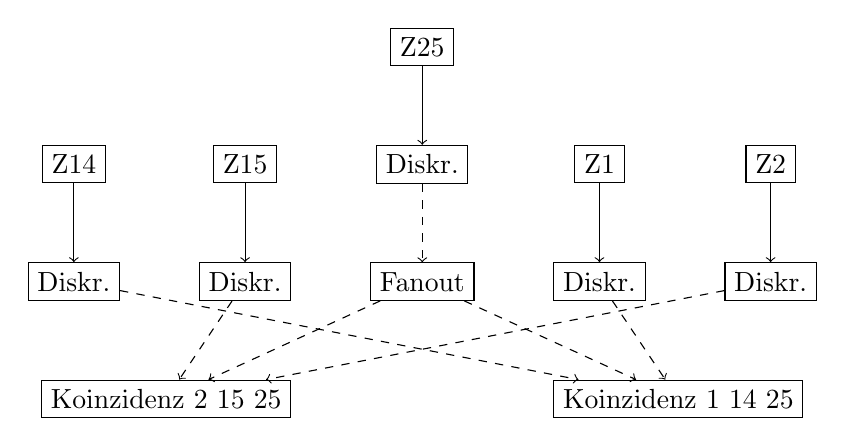
\begin{tikzpicture}
        \node[draw, rectangle] (fan) at (0, 0) {Fanout};

        \node[draw, rectangle] (D25) [above=of fan] {Diskr.};
        \node[draw, rectangle] (D1) [right=of fan] {Diskr.};
        \node[draw, rectangle] (D2) [right=of D1] {Diskr.};
        \node[draw, rectangle] (D15) [left=of fan] {Diskr.};
        \node[draw, rectangle] (D14) [left=of D15] {Diskr.};

        \node[draw, rectangle] (Z1) [above=of D1] {Z1};
        \node[draw, rectangle] (Z2) [above=of D2] {Z2};
        \node[draw, rectangle] (Z14) [above=of D14] {Z14};
        \node[draw, rectangle] (Z15) [above=of D15] {Z15};
        \node[draw, rectangle] (Z25) [above=of D25] {Z25};

        \node[draw, rectangle] (con1) [below right=of fan] {Koinzidenz 1 14 25};
        \node[draw, rectangle] (con2) [below left=of fan] {Koinzidenz 2 15 25};

        \begin{scope}[->]
            \draw (Z1) -- (D1);
            \draw (Z2) -- (D2);
            \draw (Z14) -- (D14);
            \draw (Z15) -- (D15);
            \draw (Z25) -- (D25);
        \end{scope}

        \begin{scope}[->, dashed]
            \draw (D25) -- (fan);
            
            \draw (fan) -- (con1);
            \draw (fan) -- (con2);

            \draw (D1) -- (con1);
            \draw (D14) -- (con1);

            \draw (D2) -- (con2);
            \draw (D15) -- (con2);
        \end{scope}

    \end{tikzpicture}
    \caption{%
        %
    }
    \label{fig:koinzidenz}
\end{figure}

\subsubsection{Zähler}

\section{Justierung}

\subsection{Optimieren der Verzögerung}
\label{sec:optimieren_verzoegerung}

\subsection{Einstellung der Diskriminatorschwelle}
\label{sec:einstellung_diskriminatorschwelle}

\begin{itemize}
    \item
        Gewählte Schwelle für Z12

    \item
        Anzahl Ereignisse in D12

    \item
        Anzahl der oder-Ereignisse

    \item
        Anzahl der Ereignisse in Z25

    \item
        Messdauer

    \item
        Anzahl der Koinzidenzen
\end{itemize}

% TODO Wir stellen das ganze exemplarisch für Z12 ein. Was müssen wir mit den
% anderen Zählern machen? Sind die (a) schon fertig eingestellt, (b) erhalten
% die gleichen Parameter wie Z12 oder (c) müssen jeweils noch ausgemessen
% werden?

\section{Langzeitmessung zur Winkelverteilung}
\label{sec:langzeit_winkel}

\section{Langzeitmessung des Pulshöhenspektrums}
\label{sec:langzeit_puls}

\chapter{Myonenlebensdauer}

\section{Aufbau}

\subsection{Monitorkreis}

\section{Durchführung}

\section{Auswertung}

\chapter{Ergebnis}

\end{document}

% vim: spell spelllang=de tw=79
